\documentclass{beamer}
\usepackage[english]{babel}
\usepackage[utf8]{inputenc}
\usepackage{tikz,pgfplots}
\pgfplotsset{compat=newest}
\usetikzlibrary{arrows.meta, positioning}
\usetikzlibrary{shapes.geometric}
\setbeamertemplate{navigation symbols}{}
\begin{document}

\begin{center}% complete technical system
\vspace*{2em}
  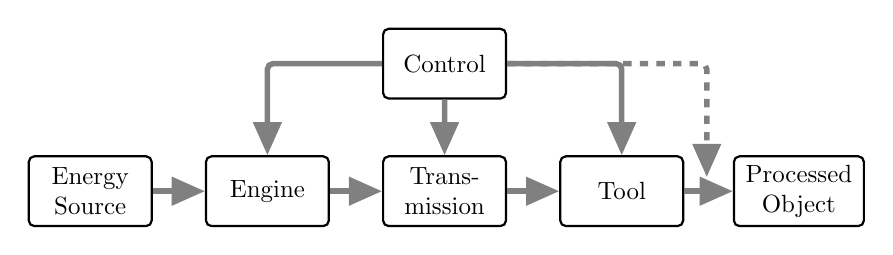
\begin{tikzpicture}[scale=.9,transform shape,
      textbox/.style={draw, text width=1.5cm, minimum height=2.8em,
        align=center},
      >={Triangle[length=0pt 6,width=0pt 5]},
      rounded corners=2pt,line width=.8pt]

    \node[textbox] at (0,0) (A1) {Energy Source};
    \node[textbox] at (2.5,0) (A2) {Engine};
    \node[textbox] at (5,0) (A3) {Trans\-mission};
    \node[textbox] at (7.5,0) (A4) {Tool};
    \node[textbox,text width=1.6cm] at (10,0) (A5) {Processed Object};
    \node[textbox] at (5,1.8) (A6) {Control};
    
    \draw[->,line width=2pt,gray] (A1) -- (A2);
    \draw[->,line width=2pt,gray] (A2) -- (A3);
    \draw[->,line width=2pt,gray] (A3) -- (A4);
    \draw[->,line width=2pt,gray] (A4) -- (A5);
    \draw[->,line width=2pt,gray] (A6) -| (A2);
    \draw[->,line width=2pt,gray] (A6) -- (A3);
    \draw[->,line width=2pt,gray] (A6) -| (A4);
    \draw[->,line width=2pt,gray,dashed] (A6) -| (8.7,0.2);
\end{tikzpicture}
\end{center}
\end{document}

\begin{center} % Almost complete technical system (without cotrol)
\vspace*{2em}
  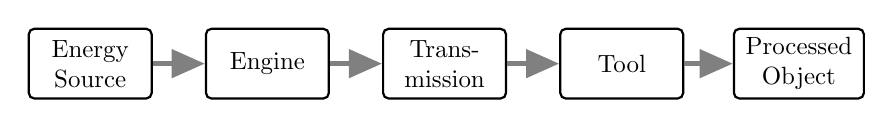
\begin{tikzpicture}[scale=.9,transform shape,
      textbox/.style={draw, text width=1.5cm, minimum height=2.8em,
        align=center},
      >={Triangle[length=0pt 6,width=0pt 5]},
      rounded corners=2pt,line width=.8pt]

    \node[textbox] at (0,0) (A1) {Energy Source};
    \node[textbox] at (2.5,0) (A2) {Engine};
    \node[textbox] at (5,0) (A3) {Trans\-mission};
    \node[textbox] at (7.5,0) (A4) {Tool};
    \node[textbox,text width=1.6cm] at (10,0) (A5) {Processed Object};
    %\node[textbox] at (5,1.8) (A6) {Control};
    
    \draw[->,line width=2pt,gray] (A1) -- (A2);
    \draw[->,line width=2pt,gray] (A2) -- (A3);
    \draw[->,line width=2pt,gray] (A3) -- (A4);
    \draw[->,line width=2pt,gray] (A4) -- (A5);
    %\draw[->,line width=2pt,gray] (A6) -| (A2);
    %\draw[->,line width=2pt,gray] (A6) -- (A3);
    %\draw[->,line width=2pt,gray] (A6) -| (A4);
    %\draw[->,line width=2pt,gray,dashed] (A6) -| (8.7,0.2);
\end{tikzpicture}
\end{center}
\end{document}

\begin{center}% flow of workpieces along the places in the tool chain.
  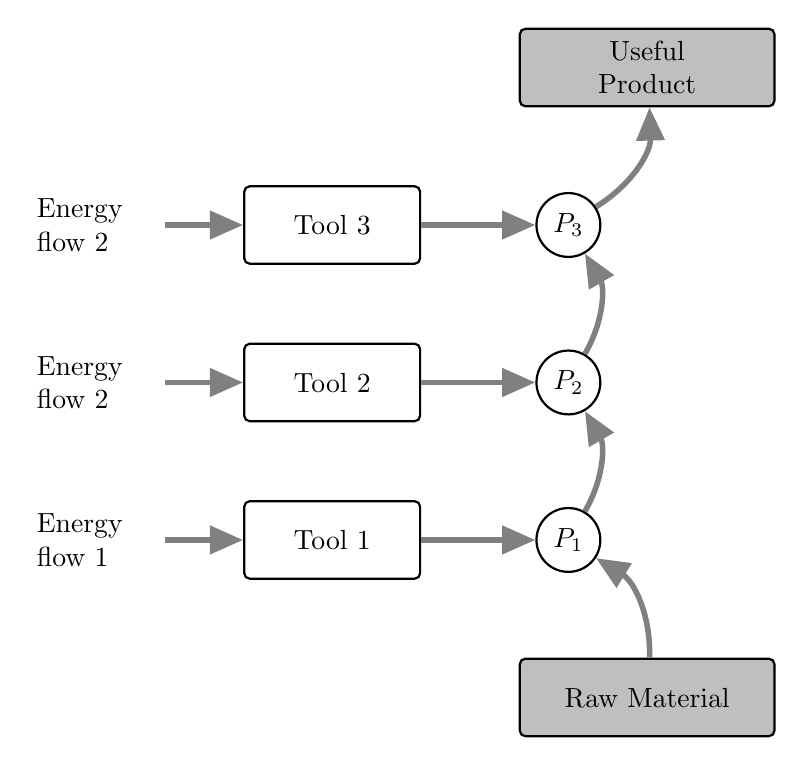
\begin{tikzpicture}[%scale=.7,transform shape,
      textbox/.style={draw, text width=3cm, minimum height=2.8em,
        align=center},
      >={Triangle[length=0pt 6,width=0pt 5]},
      rounded corners=2pt,line width=.8pt]

    \node[textbox,text width=2cm] at (1,0) (A1a) {Tool 1};
    \node[textbox,text width=2cm] at (1,2) (A1b) {Tool 2};
    \node[textbox,text width=2cm] at (1,4) (A1c) {Tool 3};
    \node[draw,circle] at (4,0) (A3a) {$P_1$};
    \node[draw,circle] at (4,2) (A3b) {$P_2$};
    \node[draw,circle] at (4,4) (A3c) {$P_3$};
    %\node[textbox] at (5,0) (A2a) {Semiproduct 1};
    %\node[textbox] at (5,2) (A2b) {Semiproduct 2};
    %\node[textbox] at (5,4) (A2c) {Semiproduct 3};
    \node[textbox,fill=lightgray] at (5,6) (A3) {Useful\\ Product};
    \node[textbox,fill=lightgray] at (5,-2) (A0) {Raw Material};
    \node[text width=1.5cm] at (-2,0) (E1) {Energy flow 1};
    \node[text width=1.5cm] at (-2,2) (E2) {Energy flow 2};
    \node[text width=1.5cm] at (-2,4) (E3) {Energy flow 2};
    
    \draw[->,line width=2pt,gray] (A1a) -- (A3a);
    \draw[->,line width=2pt,gray] (A1b) -- (A3b);
    \draw[->,line width=2pt,gray] (A1c) -- (A3c);
    \draw[->,line width=2pt,gray] (A0) to[bend right] (A3a);
    \draw[->,line width=2pt,gray] (A3a) to[bend right] (A3b);
    \draw[->,line width=2pt,gray] (A3b) to[bend right] (A3c);
    \draw[->,line width=2pt,gray] (A3c) to[bend right] (A3);
    \draw[->,line width=2pt,gray] (E1) -- (A1a);
    \draw[->,line width=2pt,gray] (E2) -- (A1b);
    \draw[->,line width=2pt,gray] (E3) -- (A1c);
\end{tikzpicture}
\end{center}

\begin{center}% minimal technical system
  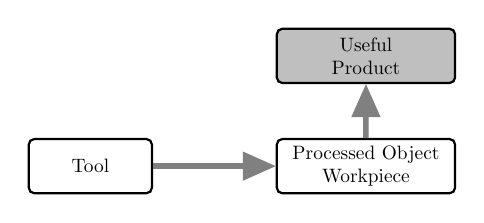
\begin{tikzpicture}[scale=.7,transform shape,
      textbox/.style={draw, text width=3cm, minimum height=2.8em,
        align=center},
      >={Triangle[length=0pt 6,width=0pt 5]},
      rounded corners=2pt,line width=.8pt]

    \node[textbox,text width=2cm] at (0,0) (A1) {Tool};
    \node[textbox] at (5,0) (A2) {Processed Object\\ Workpiece};
    \node[textbox,fill=lightgray] at (5,2) (A3) {Useful\\ Product};
    
    \draw[->,line width=2pt,gray] (A1) -- (A2);
    \draw[->,line width=2pt,gray] (A2) -- (A3);
\end{tikzpicture}
\end{center}

\begin{center}% complete technical system
  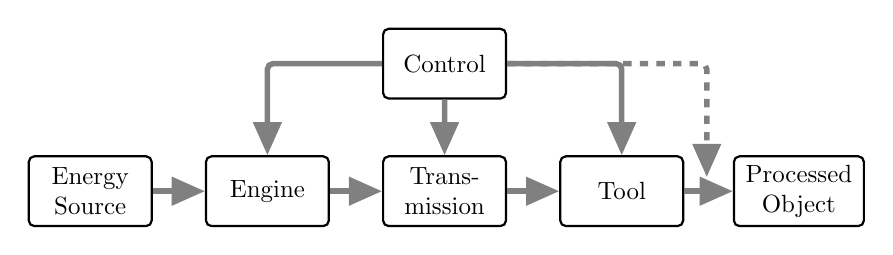
\begin{tikzpicture}[scale=.9,transform shape,
      textbox/.style={draw, text width=1.5cm, minimum height=2.8em,
        align=center},
      >={Triangle[length=0pt 6,width=0pt 5]},
      rounded corners=2pt,line width=.8pt]

    \node[textbox] at (0,0) (A1) {Energy Source};
    \node[textbox] at (2.5,0) (A2) {Engine};
    \node[textbox] at (5,0) (A3) {Trans\-mission};
    \node[textbox] at (7.5,0) (A4) {Tool};
    \node[textbox,text width=1.6cm] at (10,0) (A5) {Processed Object};
    \node[textbox] at (5,1.8) (A6) {Control};
    
    \draw[->,line width=2pt,gray] (A1) -- (A2);
    \draw[->,line width=2pt,gray] (A2) -- (A3);
    \draw[->,line width=2pt,gray] (A3) -- (A4);
    \draw[->,line width=2pt,gray] (A4) -- (A5);
    \draw[->,line width=2pt,gray] (A6) -| (A2);
    \draw[->,line width=2pt,gray] (A6) -- (A3);
    \draw[->,line width=2pt,gray] (A6) -| (A4);
    \draw[->,line width=2pt,gray,dashed] (A6) -| (8.7,0.2);
\end{tikzpicture}
\end{center}

\begin{center} % SF Model
    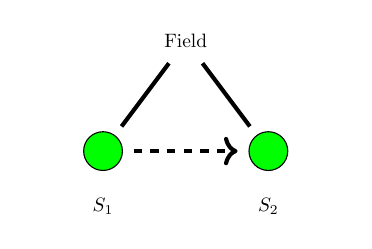
\begin{tikzpicture}[scale=.7,transform shape,
        pfeil/.style={shorten <=4pt, shorten >=4pt, line width=1.5pt},
        mytext/.style={text width=2.5cm,align=center}]
    \node[draw,fill=green,minimum size=2em] at (0,0) [circle] (A0) {};
    \node[draw,fill=green,minimum size=2em] at (3,0) [circle] (A1) {};
    \node at (1.5,2) [rectangle] (A2) {Field};
    \node[mytext,below of = A0] {$S_1$};
    \node[mytext,below of = A1] {$S_2$};
    \draw[pfeil,->,dashed] (A0)--(A1) ;
    \draw[pfeil,-] (A0)--(A2) ;
    \draw[pfeil,-] (A2)--(A1) ;
    \end{tikzpicture}
\end{center}

\begin{center} % My Six box model of TRIZ
  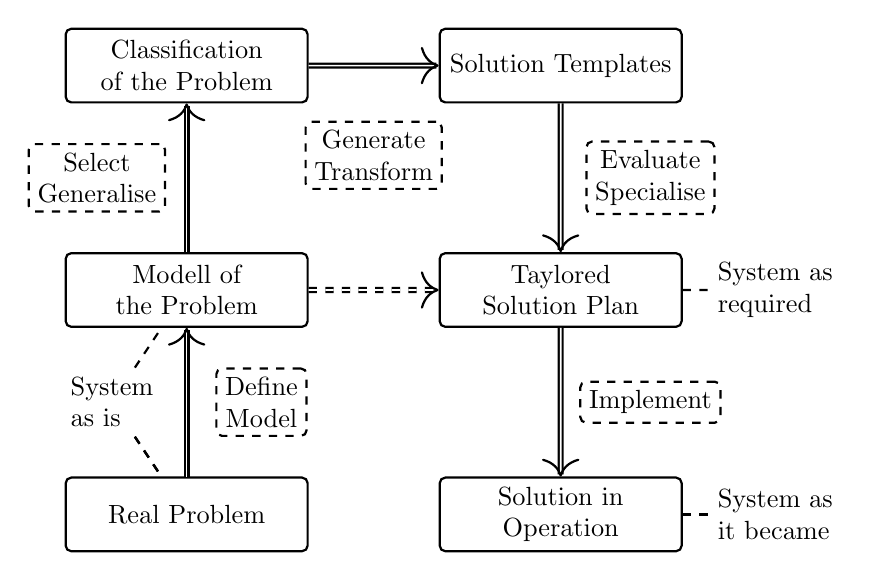
\begin{tikzpicture}[scale=.95,transform shape,
      textbox/.style={draw, text width=3cm, minimum height=2.8em,
        align=center},
      ovalbox/.style={draw, dashed, align=center},
      %>={Triangle[length=0pt 6,width=0pt 5]},
      rounded corners=2pt,line width=.8pt]

    \node[text width=1.1cm] at (-1,1.5) (A0) {System\\ as is};
    \node[textbox] at (0,0) (A1) {Real Problem};
    \node[ovalbox] at (1,1.5) {Define\\ Model}; 
    \node[textbox] at (0,3) (A2) {Modell of the Problem};
    \node[ovalbox] at (-1.2,4.5) {Select\\ Generalise}; 
    \node[textbox] at (0,6) (A3) {Classification of the Problem};
    \node[ovalbox] at (2.5,4.8) {Generate\\ Transform}; 
    \node[textbox] at (5,6) (B3) {Solution Templates};
    \node[ovalbox] at (6.2,4.5) {Evaluate\\ Specialise}; 
    \node[textbox] at (5,3) (B2) {Taylored\\ Solution Plan};
    \node[ovalbox] at (6.2,1.5) {Implement}; 
    \node[textbox] at (5,0) (B1) {Solution in Operation};
    \node[text width=1.8cm] at (8,3) (C2) {System as\\ required};
    \node[text width=1.8cm] at (8,0) (C1) {System as\\ it became};

    \draw[-,dashed] (A0) -- (A1);
    \draw[-,dashed] (A0) -- (A2);
    \draw[-,dashed] (B1) -- (C1);
    \draw[-,dashed] (B2) -- (C2);
    \draw[-,dashed] (A0) -- (A1);
    \draw[-,dashed] (A0) -- (A1);
    
    \draw[double,->] (A1) -- (A2) ;
    \draw[double,->] (A2) -- (A3) ;
    \draw[double,->] (A3) -- (B3) ;
    \draw[double,->,dashed] (A2) -- (B2) ;
    \draw[double,->] (B3) -- (B2) ;
    \draw[double,->] (B2) -- (B1) ;
  \end{tikzpicture}
\end{center}

% Car Body Department
  \begin{minipage}{.42\textwidth}\centering\vspace*{2em}
    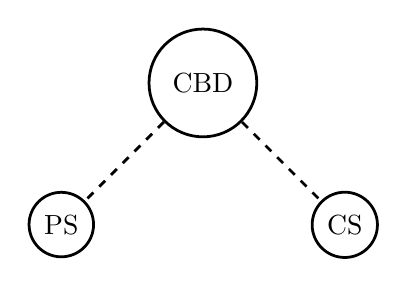
\begin{tikzpicture}[line width=1pt]
        \node[draw,text width=3em, align=center] [circle] (A0) {CBD};
        \node[draw,below left=of A0, node distance=2em] [circle] (A1) {PS};
        \node[draw,below right=of A0, node distance=2em] [circle] (A2) {CS};
        \draw[-,dashed] (A0)--(A1) ;
        \draw[-,dashed] (A0)--(A2) ;
    \end{tikzpicture}\\[2em] Structural Organisation
  \end{minipage}\hfill
  \begin{minipage}{.55\textwidth}\centering
    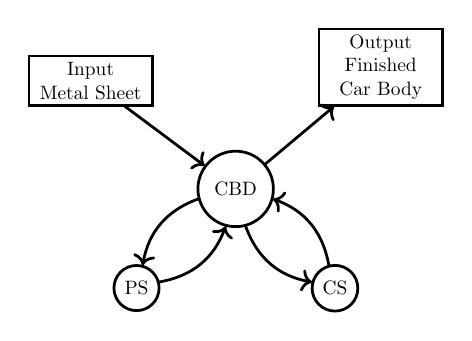
\begin{tikzpicture}[line width=1pt,scale=.7,transform shape]
    \node[draw,text width=3em, align=center] [circle] (A0) {CBD};
    \node[draw,text width=2cm, align=center, above left=of A0] [rectangle] (I)
         {Input\\Metal Sheet}; 
    \node[draw,text width=2cm, align=center, above right=of A0] [rectangle] (O)
         {Output\\Finished Car Body}; 
    \node[draw,below left=of A0, node distance=2em] [circle] (A1) {PS};
    \node[draw,below right=of A0, node distance=2em] [circle] (A2) {CS};
    \draw[->] (I)--(A0) ;
    \draw[->] (A0)--(O) ;
    \draw[->] (A0) to[bend right] (A1) ;
    \draw[->] (A1) to[bend right] (A0) ;
    \draw[->] (A0) to[bend right] (A2) ;
    \draw[->] (A2) to[bend right] (A0) ;
    \end{tikzpicture}\\[2em] Operational Organisation
  \end{minipage}

\end{document}

